\documentclass[addpoints]{exam}
\usepackage{amsmath, amsfonts}
\usepackage{forest}
\usepackage{geometry}
\usepackage{amssymb}
\usepackage{hyperref}
\usepackage{titling}
\usepackage{graphicx}
\usepackage{tikz}
\usepackage{tikz-qtree}
\usepackage{tikz-qtree-compat}
\usepackage{forest}

\printanswers

% Header and footer.
\pagestyle{headandfoot}
\runningheadrule
\runningfootrule
\runningheader{CS 212, Fall 2022}{HW 3: Turing Machines, Decidability \& Recognizabality}{\theauthor}
\runningfooter{}{Page \thepage\ of \numpages}{}
\firstpageheader{}{}{}

\boxedpoints

\title{Homework 3: Turing Machines, Decidability \& Recognizabality}
\author{Final Parser} % <=== replace with your team name
\date{CS 212 Nature of Computation\\Habib University\\Fall 2022}

\begin{document}
\maketitle

\begin{questions}

\question \label{q:lang} A Turing machine is said to \textit{compute} a function $f$ if, started with an input $x$ on its tape, it halts with $f(x)$ on its tape. Consider a binary operator $\triangle$ and a function $f$ defined as follows.
	\begin{align*}
		0\triangle 0=1, 0\triangle 1=1, 1\triangle 0=0,1\triangle 1=1\\
		f:\{0,1\}^n\times \{0,1\}^n\to \{0,1\}^n, n\in \mathbb{Z}-\mathbb{Z}^-    \\
		f(a,b) = \{ c_1c_2\ldots c_n \mid c_i = a_i\triangle b_i, i = 1,2,\ldots,n\}
	\end{align*}
	Consider the Turing machine, $M$, that computes $f$ given a $\#$-separated pair of binary strings as input. The Turing machine should print nothing if the function is undefined.

\begin{parts}
	\part[5] Give a high-level description of $M$.
	\begin{solution}
		We build a turing machine $M$ that computes $f$ the idea is on input $a\#b$ we first count if length of $a$ is equal to length of $b$ if not we remove everything from the tape and reject.
    \\If lenght of $a$ and $b$ are equal then we place a \# at the end of out strinf and start writing $c$ after the hash. We compute $c$ by first readind $i^{th}$ symbol from $a$ then $b$ and then computing the corresponding $i^{th}$ symbol for $c$ and writing it in $c$.
    \\Once done we erase everything other than $c$ from the tape and accept.
		\\The high level description of the machine \(M\) is, 
    \\let \(M=\)``On input \(a\#b\), where \(a\) and \(b\) are binary strings,
		\begin{enumerate}
			\item Mark the first symbol if you read 0 then mark $0_s$ if read 1 then read mark it is as $1_s$. Return to start of the tape.
			\item If you read 0 mark it as $\overline{0}$, if you read 1 mark it as $\overline{1}$, if you read $0_s$ mark it as $\overline{0}_s$, if you read $1_s$ mark it as $\overline{1}_s$.
			\item Move right until \# is read.
			\item Move right until 0 or 1 is read, if 0 is read mark it as $\overline{0}$, if 1 is read mark it as $\overline{1}$. If no 0 or 1 are found then, return to the start of the tape, replace every non-$\sqcup$ symbol with $\sqcup$ and then \textit{reject}.
			\item Move left until \# is read, then move left until first $\overline{0}$ or $\overline{1}$ is read. If symbol to left is 0 or 1 then return to step 2, else move to next step.
			\item If next symbol is \# then move until you keep reading $\overline{0}$ or $\overline{1}$, if there are still 0 or 1 remaining on the tape towards the right side of the head, then return to the start of the tape, replace every non-$\sqcup$ symbol with $\sqcup$ and then \textit{reject}. Else move left until $\sqcup$ is read replace it with a \# and move to next step.
			\item Return to start of the tape. 
			\item Move right until a non-$\sqcup$ symbol is read.
			\item If $\overline{0}$ or $\overline{0}_s$ is read, replace it with $\sqcup$ and move right until \# is read then move right until $\overline{0}$ or $\overline{1}$ are read. Replace it with $\sqcup$ and move right until \# if read, then move right until $\sqcup$ is read and replace it with 1. Then return step 7.
			\item If $\overline{1}$ or $\overline{1}_s$ is read, replace it with $\sqcup$ and move right until \# is read then move right until $\overline{0}$ or $\overline{1}$ are read. If $\overline{0}$ is read replace it with $\sqcup$ and move right until \# if read, then move right until $\sqcup$ is read and replace it with 0.  Else if $\overline{1}$ is read replace it with $\sqcup$ and move right until \# if read, then move right until $\sqcup$ is read and replace it with 1. Then return step 7.
			\item If \# is read replace it with $\sqcup$ move right until \# is read replace it with $\sqcup$. \textit{accept}.
		\end{enumerate}
	\end{solution}

	\newpage

	\part[5] Give a formal description of $M$, expressing the transition function, $\delta$, as a state diagram that shows all the transitions.
	\begin{solution}
		We can express the transition function, $\delta$, as a state diagram that shows all the transitions. The diagram is as follows.

		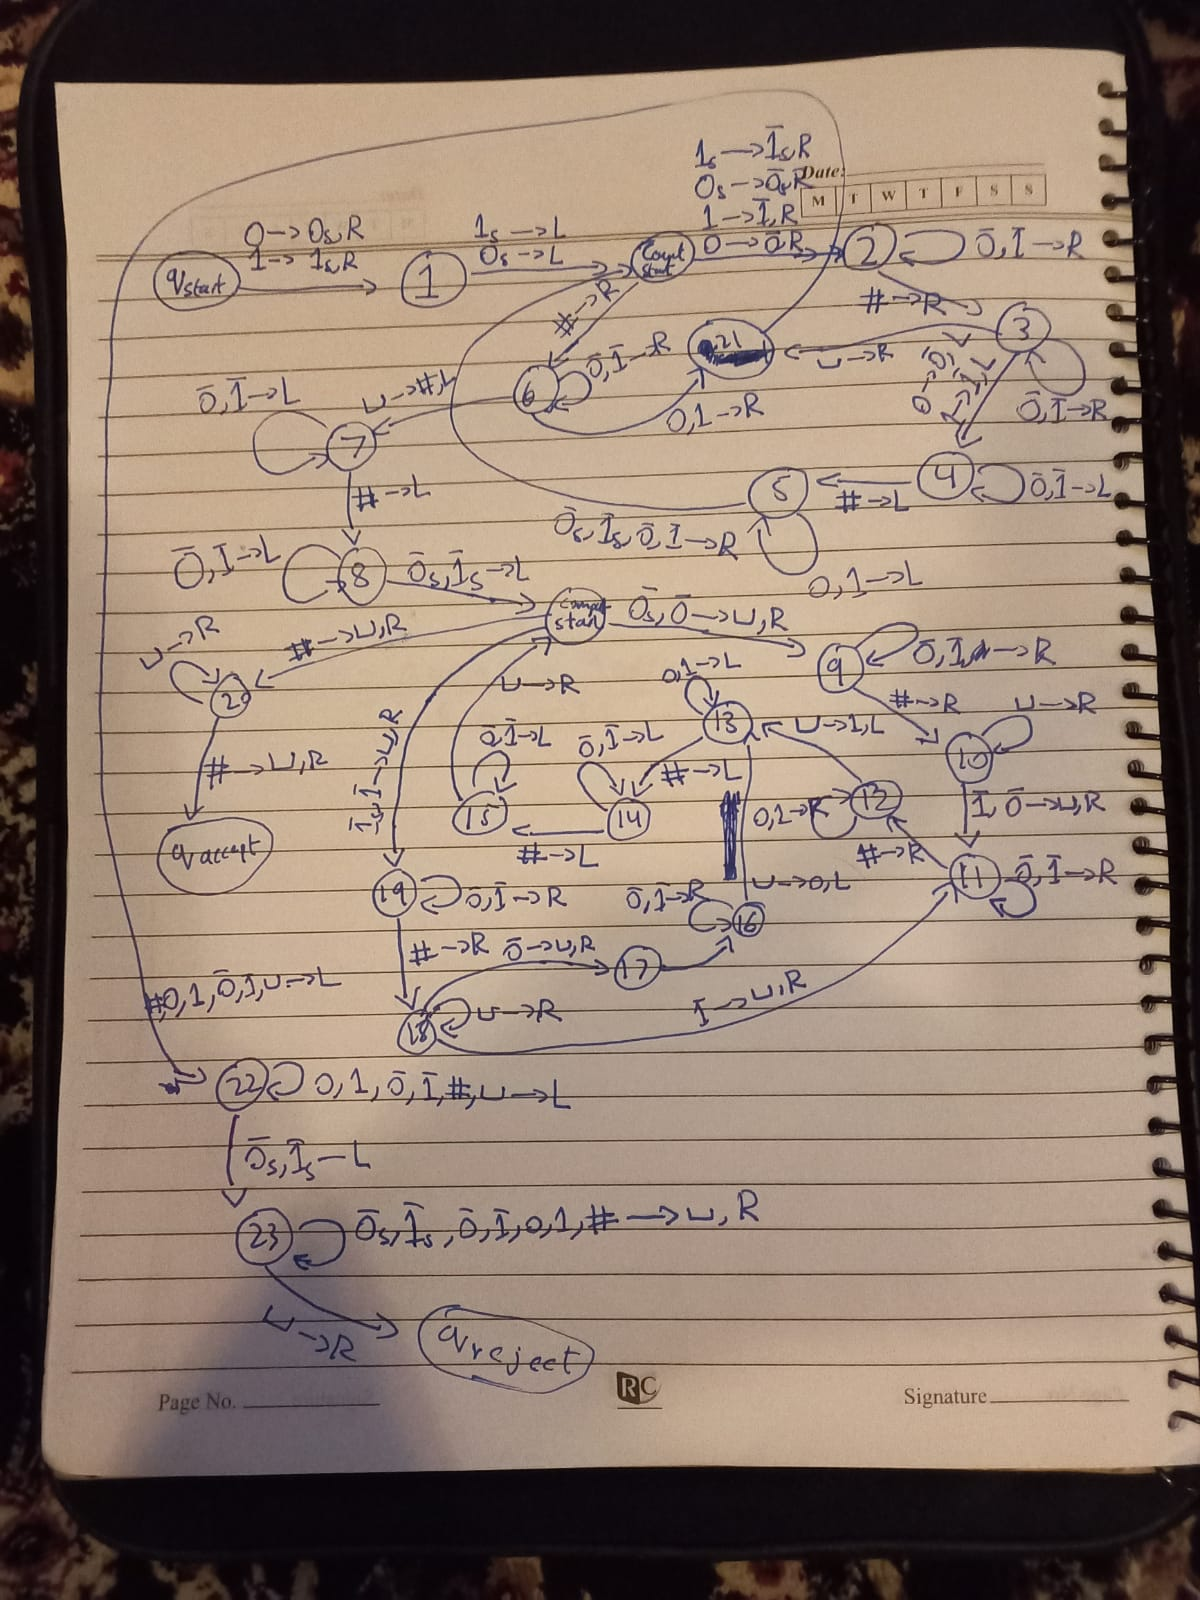
\includegraphics[width=0.9\textwidth]{pic.jpeg}
	\end{solution}

	\end{parts}

	\newpage

\question [10] An $\textit{Euclidean-Space}$ Turing machine has the usual finite-state control but a tape that extends in a three-dimensional grid of cells, infinite in all directions. Both the head and the first input symbol are initially placed at a cell designated as the origin. Each consecutive input symbol is in one of the six neighboring cells and does not overwrite a previous symbol. The head can move in one transition to any of the six neighboring cells. All other workings of the Turing machine are as usual. Provide a formal description of the \textit{Euclidean-Space} Turing Machine and prove that it is equivalent to an ordinary Turing machine. Recall that two models are equivalent if each can simulate the other.
	\begin{solution}
    We show that the Euclidean-Space Turing machine is equivalent to the normal Turing machine, by first showing that the Euclidean-Space Turing machine can simulate a Turing machine and a Turing machine can simulate Euclidean-Space Turing machine. (We use Turing machine here for a a normal Turing machine as described in Definition 3.3 of the book).
		\\Let $E$ be a Euclidean-Space Turing machine and $M$ be a Turing Machine. 
    \\First we show that $E$ can simulate $M$. This is trivial as for $E$ to simulate $M$ it just need to keep moving in the position $x$ axis (right of the origin cell). And just use the line of cells that extend in the direction of the positive $x$ axis from the origin. This way $E$ can simulate $M$.
    \\For $M$ to simulate $E$, lets say we assign a number $n \in \mathbb{N}$ to each cell in the tape of $M$ starting from 0, where the left most cell is assigned 0 the cell next to it is 1, the one next to that is 2 and so on.
    \\Now cell 0 represent $M$ represent the cell starting cell in $E$. 
    \\Now for transition in $E$ where you move from starting cell to cell right to it in $M$ you move from cell 0 to cell $6\times 0 + 1 = 1$.
    \\For transition in $E$ where you move from starting cell to cell above it in $M$ you move from cell 0 to cell $6\times 0 + 2 = 2$.
    \\For transition in $E$ where you move from starting cell to cell in front of it in $M$ you move from cell 0 to cell $6\times 0 + 3 = 3$.
    \\For transition in $E$ where you move from starting cell to cell left to it in $M$ you move from cell 0 to cell $6\times 0 + 4 = 4$.
    \\For transition in $E$ where you move from starting cell to cell below it in $M$ you move from cell 0 to cell $6\times 0 + 5 = 5$.
    \\For transition in $E$ where you move from starting cell to cell at the back of it in $M$ you move from cell 0 to cell $6\times 0 + 6 = 6$.
    \\Using this idea if you are at a cell labeled $n$ in $M$ and the transition in $E$ moves head to right, then on $M$ move to cell $6\times n + 1$.
    \\If you are at a cell labeled $n$ in $M$ and the transition in $E$ moves head above, then on $M$ move to cell $6\times n + 2$.
    \\If you are at a cell labeled $n$ in $M$ and the transition in $E$ moves head forward, then on $M$ move to cell $6\times n + 3$.
    \\If you are at a cell labeled $n$ in $M$ and the transition in $E$ moves head to left, then on $M$ move to cell $6\times n + 4$.
    \\If you are at a cell labeled $n$ in $M$ and the transition in $E$ moves head below, then on $M$ move to cell $6\times n + 5$.
    \\If you are at a cell labeled $n$ in $M$ and the transition in $E$ moves head backwards, then on $M$ move to cell $6\times n + 6$.
    \\This way $M$ can simulate $E$.
    \\As we have shown that a Euclidean-Space Turing machine can simulate a Turing machine and a Turing machine can simulate a Euclidean-Space Turing machine, we have that the Euclidean-Space Turing machine is equivalent to the Turing Machine.
    \hfill\(\blacksquare\)
	
  \end{solution}

\question [10] Theorem 4.5 in our textbook states that $EQ_{DFA}$ is decidable. Formally define $EQ_{PDA}$ and prove that if it is undecidable, it is also unrecognizable. 
\begin{solution}
  	We define $EQ_{\mbox{PDA}}$ as follows,
	\[
		EQ_{\mbox{PDA}} = \{\langle A,B\rangle|A\mbox{ and } B \mbox{ are DFAs and }L(A)=L(B)\}
	\]
	We show that $\overline{EQ}_{\mbox{PDA}} $ is recognizable. We build a Turing machine $T$ that recognizes $\overline{EQ}_{\mbox{PDA}}$. Let $T$ = ``On input $\langle P_1, P_2\rangle$, where $P_1$ and $P_2$ are 2 PDAs
    \begin{enumerate}
      	\item Generate a string $w \in \Sigma^*$, where $\Sigma$ is the alphabet of $P_1$ and $P_2$
		\item Simulate $P_1$ on $w$
		\item Simulate $P_2$ on $w$
		\item If $P_1$ accepts and $P_2$ doesn't accept then \textit{accept}. Else if $P_2$ accepts and $P_1$ doesn't accept then \textit{accept}. Else if $P_2$ doesn't accept and $P_1$ doesn't accept then go back to step 1. Else if $P_1$ accepts and $P_2$ accepts then go back to step 1."
    \end{enumerate}
    Given that $EQ_{\mbox{PDA}}$  is undecidable. As we know $EQ_{\mbox{PDA}}$ is undecidable and $\overline{EQ}_{\mbox{PDA}}$ is recognizable from THEOREM 4.22 of the book, we have that $EQ_{\mbox{PDA}}$ is unrecognizable.
\end{solution}

\question [10] Let $A = \{L \mid L\text{ is decidable but not context-free}\}$. Prove that every element of $A$ contains an unrecognizable subset.
\begin{solution}
	Let $L\in A$, as every finite language is context-free, and $L$ is not context free then $L$ is infinite.

	The set of all subsets of $L$ is the power set $\mathcal{P}(L)$. We know from Cantor's Theorem that $|L| < |\mathcal{P}(L)|$ . If $L$ is an infinite set then as from  $|L| < |\mathcal{P}(L)|$ we know $\mathcal{P}(L)$ must be uncountable. From COROLLARY 4.18 from the book we know that the set of all Turing machine is countable. And as the set of all subsets of $L$ is uncountable, then there must be some subset of $L$ for which a Turing machine doesn't exist (from Cantor's Theorem).

	Therefore for every element $L$ of $A$, $L$ has an unrecognizable subset. \hfill $\blacksquare$
\end{solution}

\end{questions}

\end{document}

%%% Local Variables:
%%% mode: latex
%%% TeX-master: t
%%% End:
